\chapter{評価スコアを推定するモデルの構築}
\thispagestyle{myheadings}
\label{chap:model}

本章では,UTAU音源ライブラリに対して声質に対する評価スコアを付与するための機械学習モデルの概要と実装について述べる.
\ref{sec:utau}節では推論に用いるUTAU音源ライブラリとUTAU音源声質アンケートについて述べる.
\ref{sec:feature}節では使用する音声ファイルと音響特徴量,その抽出方法について述べる.
\ref{sec:model}節では評価スコアを推論する機械学習モデルの構築について述べ,\ref{sec:eval}節で構築したモデルの精度を評価する.

\section{UTAU音源ライブラリとUTAU音源声質アンケート}
\label{sec:utau}

本研究において探索対象とするUTAU音源ライブラリと,声質評価の基準及び学習データとして用いるUTAU音源声質アンケートについて説明する.
UTAU音源ライブラリはwavファイルとメタデータを含むファイル群からなるデータセットであり,UTAU音源ファイルとして提供される.
wavファイルの中身は収録方式によって多少異なるが,現在広く用いられている連続音方式であれば「あんああいあうあ」\cite{tatsu3shiki}といった形で複数の音素をできる限り一定の音程と音量になるように収録された肉声がwavファイルとして保存されいる.
図\ref{fig:utau_files}で実際のUTAU音源ライブラリの一部を示す.
個人が作成・公開が可能で,ソフトと同じく無償で公開されているものが多い.
UTAUは波形接続と呼ばれる手法を用いており,この音声データを切り貼りして加工し,歌声を合成する.

\begin{figure}[htb]
  \centering
  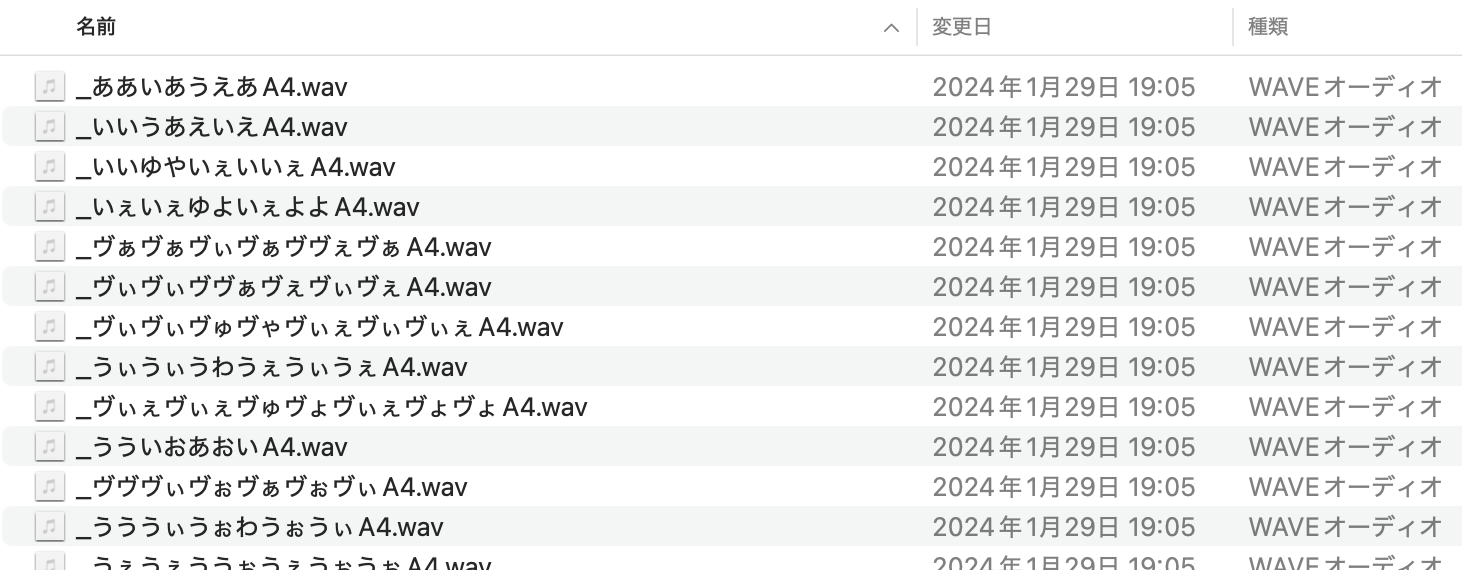
\includegraphics[width=0.9\textwidth]{fig/utau_files.png}
  \caption{UTAU音源ファイルの一部}
  \label{fig:utau_files}
\end{figure}

UTAU音源声質アンケートはニコニコ大百科上で提言されたUTAU音源ライブラリに対してその声の特徴を評価するためのアンケート規格であり\cite{utausurvey},現在までにこの規格を用いて250種以上のUTAU音源ライブラリに対してアンケートが行われている.
このアンケート規格では,UTAU音源の声に対して表\ref{tab:survey}に示す7項目について,それぞれ1から7までの7段階評価で10件以上のアンケート調査を行い,その平均を評価値とするとされている.
実際のアンケートの実施方法や具体的な集計件数は定められておらず,アンケートの実施者が各自で決め行っている.

\begin{table}[htb]
  \centering
  \caption{UTAU音源声質アンケートの評価軸}
  \label{tab:survey}
  \begin{tabular}{c|cc}
    \hline
    評価軸 & 低い値の示す表現語 & 高い値の示す表現語 \\
    \hline
    声の性別 & 女性的 & 男性的 \\
    滑舌 & 舌足らず & はきはき \\
    特有性 & 素直 & 癖がある \\
    声の年齢 & 幼い & 大人びた \\
    透明感 & ノイジー & クリア \\
    声の強さ & 優しい & 力強い \\
    声の明度 & 暗い & 明るい \\
    \hline
  \end{tabular}
\end{table}

\section{特徴量の抽出}
\label{sec:feature}

UTAU音源ライブラリから推論に用いる音響特徴量を抽出する方法について述べる.
特徴量の抽出には,UTAU音源ライブラリから複数の音階で「あ」「い」「う」「え」「お」「ん」と発声した音声をライブラリ中の音声ファイルを直接操作して作成し,利用する.
これらの音素を選択した理由は,五母音と子音「ん」が継続的に発声可能な音素であり,安定した音声区間から音響特徴を効果的に抽出できるためである.
音声ファイルの操作には,ライブラリに「固定範囲外」として指定される範囲を利用した.
図\ref{tab:waveform}に「あ」を発声している音声ファイルの波形とスペクトログラム,ライブラリに指定されるタイミングの例を示す.
この図はUTAU互換ソフトウェアであるOpenUTAUからキャプチャしたものである.
波形上の白色の背景の範囲が固定範囲外であり,UTAUが実際に音声の合成を行う際は母音を伸ばすためにこの範囲の音声を加工している.
固定範囲外は音素の発声始めと終わりの部分を含まないため,発声とひいては音声波形・スペクトログラムの形状が安定しており,音声の特徴を抽出しやすいと考え,この音声区間を用いた.
音声の評価には各音素の発声を5つの音階ごとに生成した.
歌唱において現実的に使用されると考えた表\ref{tab:hz}に示すA3〜F5の5音階を用い,対応する周波数へピッチシフト処理を行い声高を変更し生成した.
複数の音階の利用には,特徴量の数を増やし機械学習モデルの精度向上を図る目的のほか,多音源音源と呼ばれる複数の音階で収録された音声ファイルを持つUTAU音源ライブラリへの対応が目的として存在する.
多音階音源では歌声を合成する際,合成目標の声高に近い音階の音声を加工するため声高の変更による劣化を抑え,より自然な声を合成できる.
特徴量抽出のためのピッチシフト処理においても,この多音階音源の仕様を考慮し適切な音声ファイルを選択し加工している.
この音域ごとの音源ファイルの切り替えによる声質の変化を特徴量として捉え,多音階音源に対しより適切な評価スコアを推論できると考えた.

\begin{figure}[htb]
  \centering
  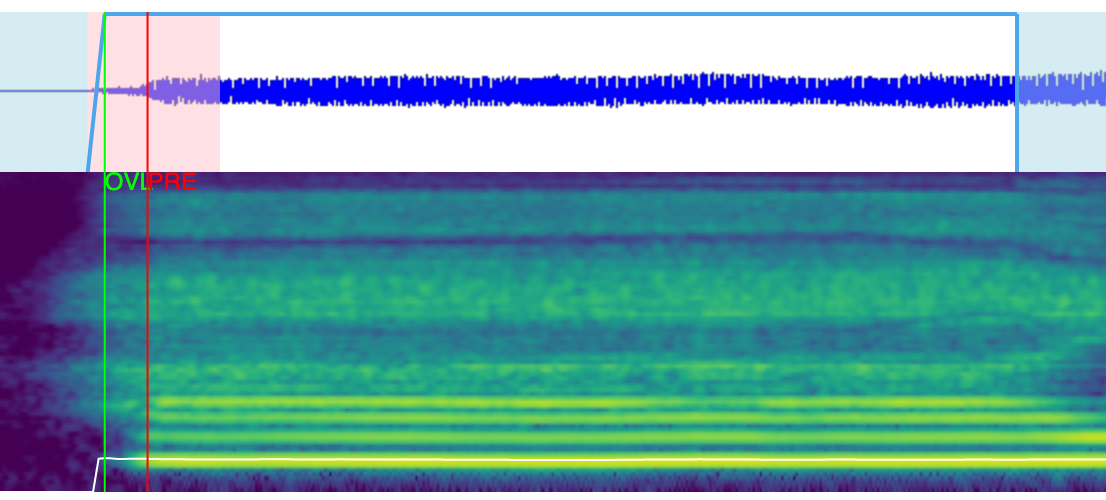
\includegraphics[width=0.9\linewidth]{fig/eve_a.png}
  \caption{音声ファイルの波形とスペクトログラム,ライブラリに指定されるタイミング}
  \label{tab:waveform}
\end{figure}

\begin{table}[htb]
  \centering
  \caption{使用する音階とHzの対応表}
  \label{tab:hz}
  \begin{tabular}{c|c}
    \hline
    音階 & 周波数(Hz) \\
    \hline
    A3 & 220.000 \\
    D4 & 261.626 \\
    G4 & 391.995 \\
    C5 & 523.251 \\
    F5 & 698.456 \\
    \hline
  \end{tabular}
\end{table}

実際に用いる特徴量としては,MFCC,ZCR,F1〜F4の周波数を採用した.
Pythonライブラリであるlibrosaを用いて各音階と音素ごとにこれらの特徴量を抽出し,評価スコアの推論に用いた.
librosaは音声信号処理のためのライブラリであり,音声ファイルを読み込み,スペクトログラムやMFCCなどの音響特徴量を抽出する機能を提供している.
今回設定した音響特徴量を全て抽出できるライブラリであり,またPythonでの利用が容易であるため採用した.
表\ref{fig:mfcc}に実際に抽出した特徴量の一部を示す.
以下にそれぞれの特徴量についてとその採用理由について説明する.

\begin{table}[htb]
  \centering
  \caption{実際に抽出した特徴量の一部}
  \label{fig:mfcc}
  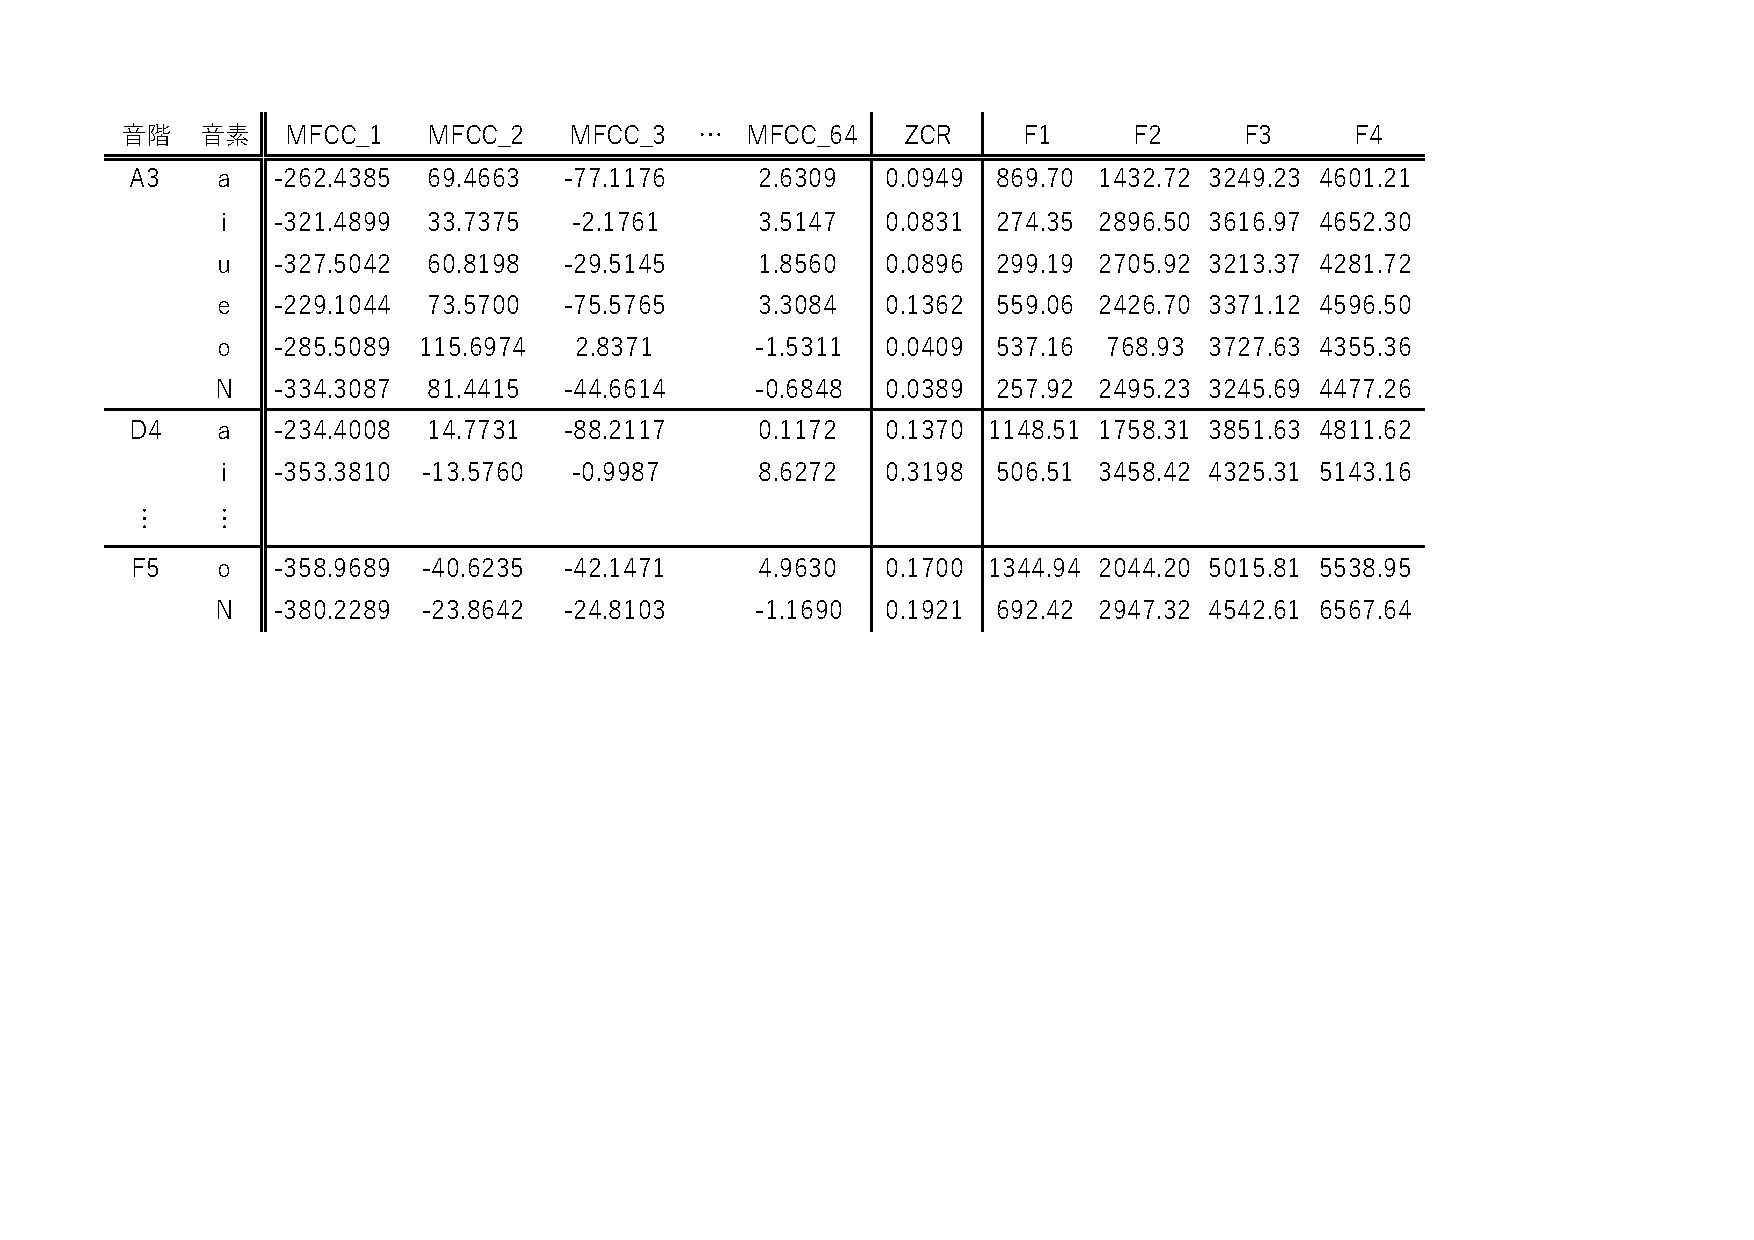
\includegraphics[width=0.9\linewidth]{fig/features_sample_ama.pdf}
\end{table}

MFCCはメル周波数ケプストラム係数の略で,音声の周波数成分を人間の聴覚特性に基づいて変換した数列である.
音声信号に対してフーリエ変換を適用して得られる周波数スペクトルを,人間の聴覚特性に合わせて変換(メルスケール変換)し,さらに対数変換と離散コサイン変換を適用して得られる.
周波数スペクトルと比較してMFCCは聴覚特性に合わせた特徴量を持つため,人間からの聞こえ方の特徴をよく反映しており,小島らによる歌声の印象評価と音響特徴量の関係についての研究\cite{mfcc_cute}ではMFCCが歌声の声質評価に有用だと示されている.
声質の特徴に大きな影響があると考え,本研究では生成した音声からMFCCを64次元まで取得し特徴量として用いた.

ZCRは音声の波形が0を交差する頻度を表す指標であり,音声信号の時間軸上で波形が正から負,または負から正に変化する回数を示す.
高い音声ほど周波数が高くなり波形の変化が多くなるためZCRも高くなるほか,摩擦音のような雑音成分が多い音声でもZCRは高くなる.
音声の声高を固定した今回の音声であれば,音声の透明感などに関連する指標として扱えると考え採用した.

フォルマントは周波数スペクトルのピークの周波数であり,周波数の低いものから順にF1,F2,と言った具合に呼ばれる.
フォルマントは声質や音素の音色に大きく関係する特徴量で特に母音の認識に重要とされており,音声の母音によってそのフォルマント周波数には一定の傾向がある.
粕谷らの研究によれば,同じ母音のフォルマント周波数でも話者の年齢や性別によって変化があり\cite{formant},声の性別感や年齢感に影響があると考えられる.
それらの特徴の表現に期待し,本研究ではF1〜F4のフォルマント周波数を特徴量として採用した.

\section{モデルの構築}
\label{sec:model}

モデルの構築にはPythonライブラリであるPyCaretを用いた.
PyCaretは機械学習のワークフローを簡略化するAutoMLライブラリのひとつである.
少ないコード量で機械学習のプロセスを実行でき,また様々な機械学習モデルを効率的に比較・評価し,最適なモデルを構築出来るためこのライブラリを採用した.
各評価スコアを推論の目標として与え,先述の特徴量から評価スコアを推定するモデルを評価スコアの7軸それぞれについて別々に作成した.

スコアの教師データにはUTAU音源声質アンケートの結果を用いた.
UTAU音源声質アンケートの結果は各ライブラリごとのニコニコ大百科記事や,配布ページなどで掲載されているほか,それらを取りまとめたデータがExcelファイルとして提供されており,本研究ではこのデータを利用した.
ファイルに記載されている240種のUTAU音源ライブラリのうち,現在でもダウンロードが可能であり,必要な音素が収録されていて,かつ利用規約上で研究目的を含む機械学習用途での利用が禁止されていない168ライブラリを学習対象とした.
データセットは学習データとテストデータに分割し,ランダムに選択した30\%をテストデータ,残りの70\%を学習データとして使用した.

7つの評価軸それぞれについてPyCaretで選択できるモデルごとのR2値を主な指標に推定精度を比較した結果,全体的に精度の優れていたAdaBoost Regressorを選択した.
R2値は決定係数とも呼ばれ,回帰分析の際に推論の精度を示す指標である.
AdaBoost Regressorはアンサンブル学習の一種であり,複数の弱学習器を組み合わせて強学習器を構築する手法である.
弱学習機としては決定木を用いており,学習データの誤差を修正するために学習データの重みを調整しながら学習を行う.
他のモデルではExtra Trees Regressorが比較時高い精度を示したが,学習後の結果を見ると過学習の傾向が見られた.
比較時のR2値の高さに加え,学習後の結果を見ても過学習の傾向が見られなかったため,本研究ではこのモデルを採用した.

\section{結果の評価}
\label{sec:eval}

構築したモデルによる推論の精度を評価するため,テストデータに対して推論を行い得た値と実際のアンケートによって得られた値を比較する.
テストデータは先述の通り学習データから各評価軸ごとにランダムに選ばれたデータであり,対象とした168ライブラリの3割にあたる51ライブラリを用いた.

図\ref{tab:score_box}では,横軸は評価軸を,縦軸はテストデータにおける実際の値と推測された値とのRMSE(Root Mean Square Error: 二乗平均平方根誤差)を,エラーバーは誤差の標準偏差を示している.
RMSEは実際の値と推測された値の差を二乗して平均を取った後に平方根を求めたもので,数値予測モデルの精度を評価する際によく用いられる指標である.
結果を見ると,RMSEの最も小さい「滑舌」の軸では0.72,最も大きい「声の性別」の軸では1.27を示しており,評価軸ごとに大きな差は見られなかった.
RMSEは0に近いほど予測精度の高さを示し,評価スコアが1から7の数値を取る点を考慮すると,全体的に中程度の精度が得られたと言える.
RMSEの平均は0.98となり,この結果は先行研究\cite{dnn}での報告値0.96に近く,音響特徴量を用いた機械学習モデルとして一定の妥当性を示した.

\begin{figure}[htb]
  \centering
  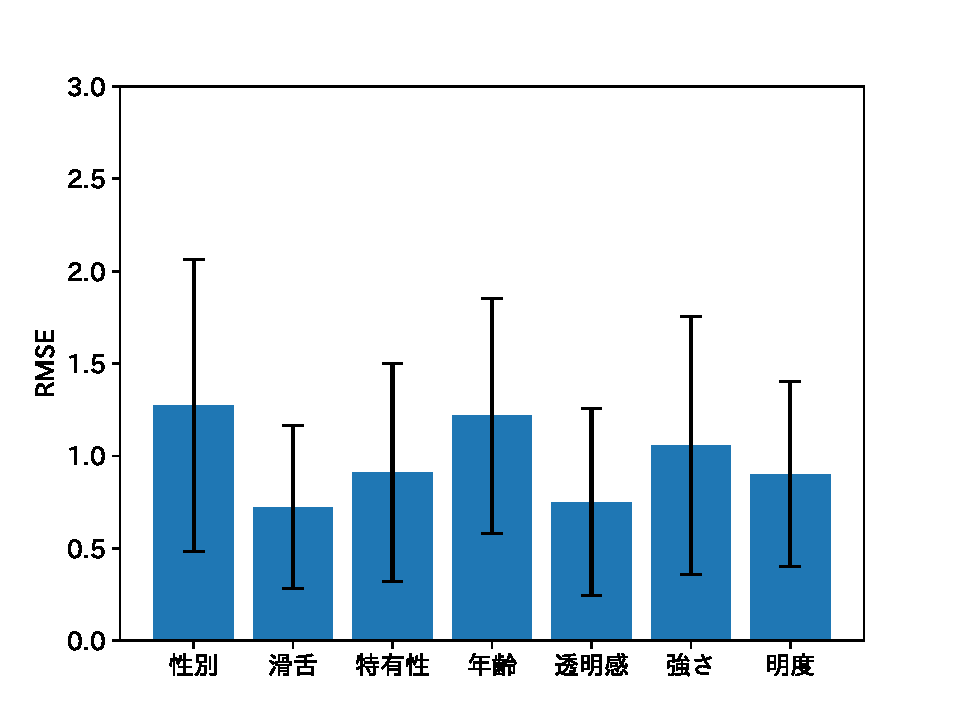
\includegraphics[width=\linewidth]{fig/rmse.pdf}
  \caption{テストデータとの誤差の二乗平均平方根}
  \label{tab:score_box}
\end{figure}

図\ref{tab:score_coor}では,横軸は評価軸を,縦軸はテストデータにおける実際の値と推測された値との相関係数を示している.
各軸ごとの相関係数を見ると,最も低い「声の年齢」は0.20とかなり低いものの,他の評価軸では0.49から0.66程度,最も高い「声の強さ」では0.66であった.
この結果から,声質の評価スコアを音響特徴量から推測するモデルが一定の相関を持っていることが分かる.

\begin{figure}[htb]
  \centering
  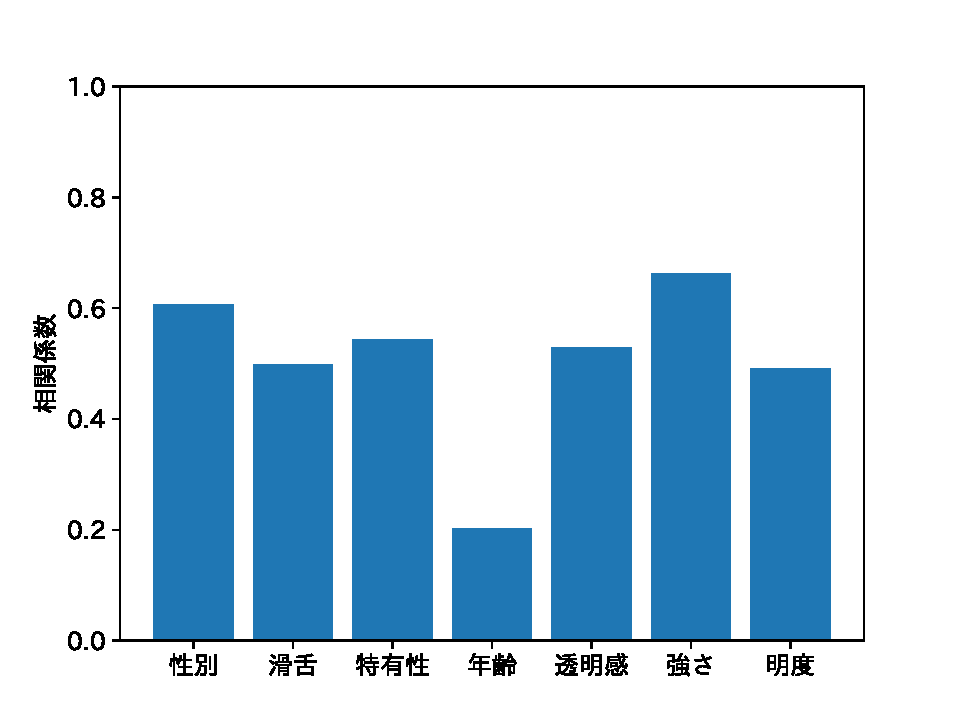
\includegraphics[width=\linewidth]{fig/coorpdf.pdf}
  \caption{テストデータとの相関係数}
  \label{tab:score_coor}
\end{figure}

7つの評価軸ごとの予測された値と実際の値との散布図を図\ref{fig:scatters}に示す.
図を見ると,相関係数の高かった「声の強さ」は右肩上がりの傾向が見られ相関の存在が分かる一方で,最も低かった「声の年齢」では点が縦に長く分布している傾向が分かる.
これは相関の弱さだけでなく,実際の値はスコア範囲中に広く分布しているにも関わらず,予測された値がおおよそ3〜5と範囲の中央に偏っている現状を示している.
このような傾向は程度の差はあるものの他の評価軸でも見られ,精度を下げてる一因となっている.

\begin{figure}[htb]
  \centering
  \subcaptionbox{声の性別}{
  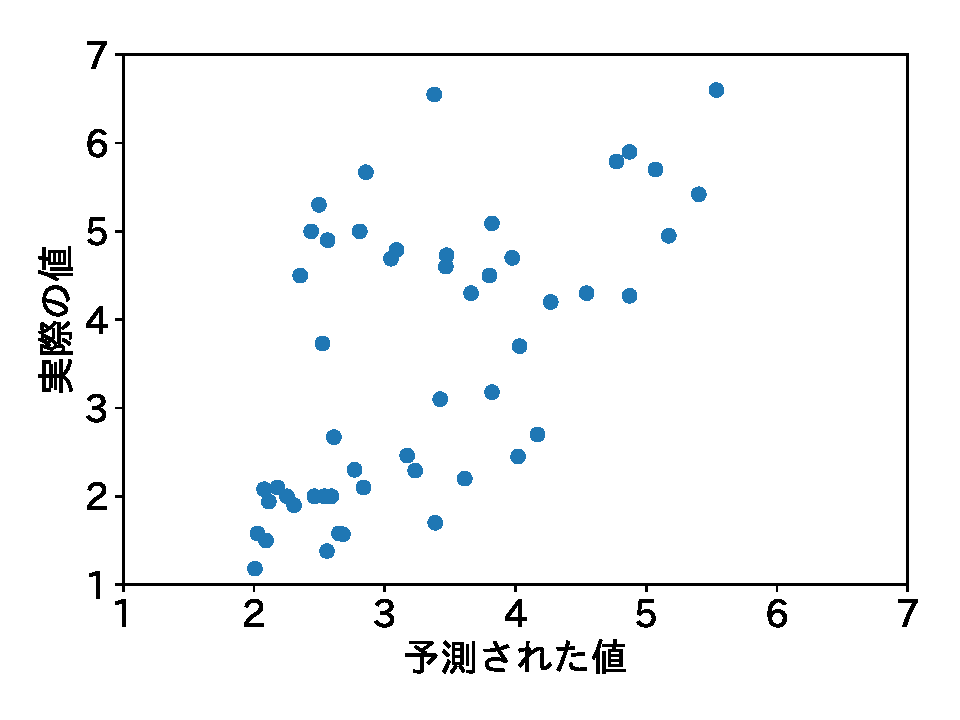
\includegraphics[width=0.4\linewidth]{fig/scatter/0.pdf}}
  \hspace{3mm}
  \subcaptionbox{滑舌}{
  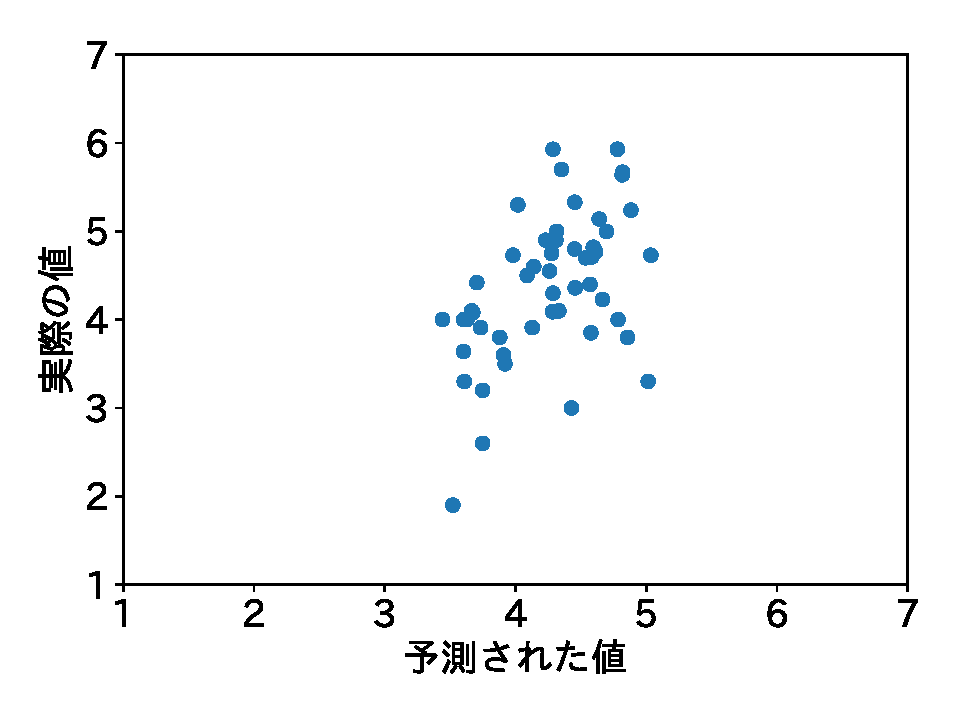
\includegraphics[width=0.4\linewidth]{fig/scatter/1.pdf}}
  \vspace{3mm}
  \subcaptionbox{特有性}{
  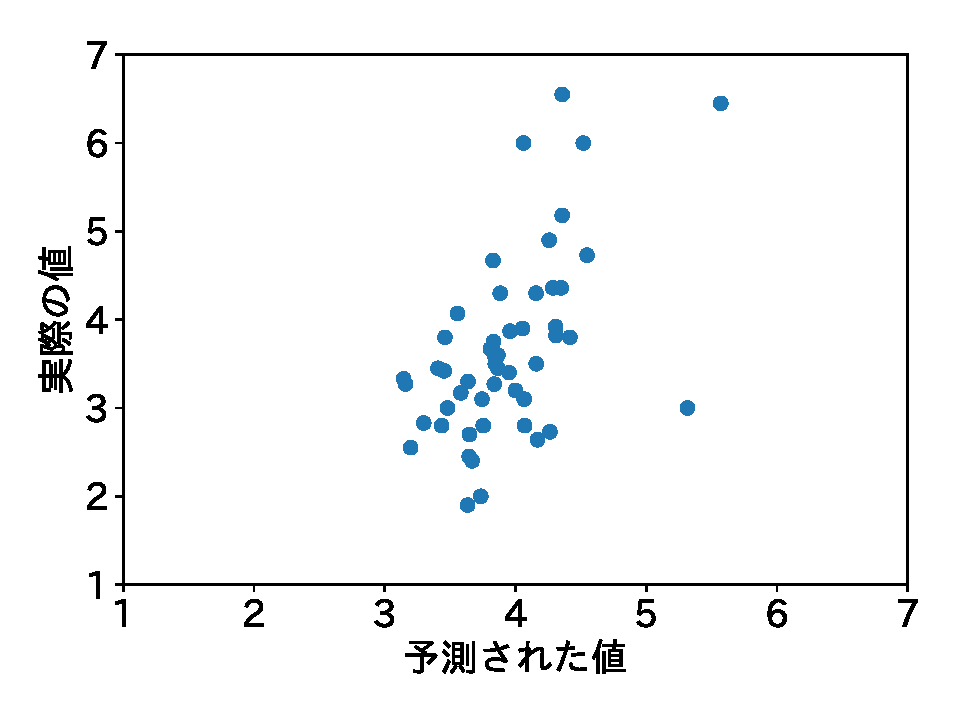
\includegraphics[width=0.4\linewidth]{fig/scatter/2.pdf}}
  \hspace{3mm}
  \subcaptionbox{声の年齢}{
  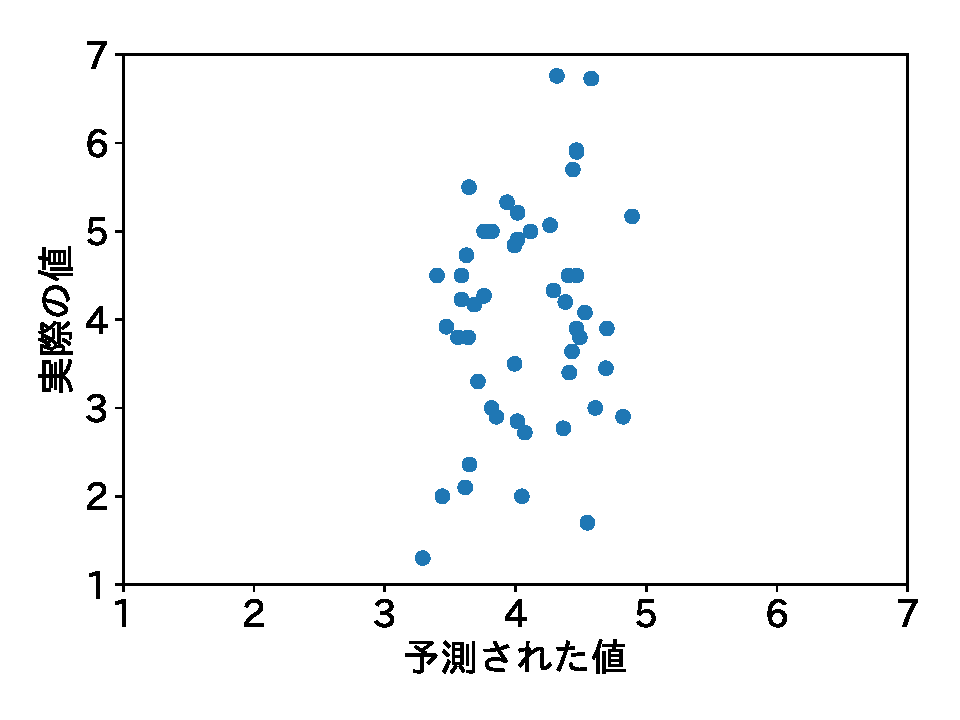
\includegraphics[width=0.4\linewidth]{fig/scatter/3.pdf}}
  \vspace{3mm}
  \subcaptionbox{透明感}{
  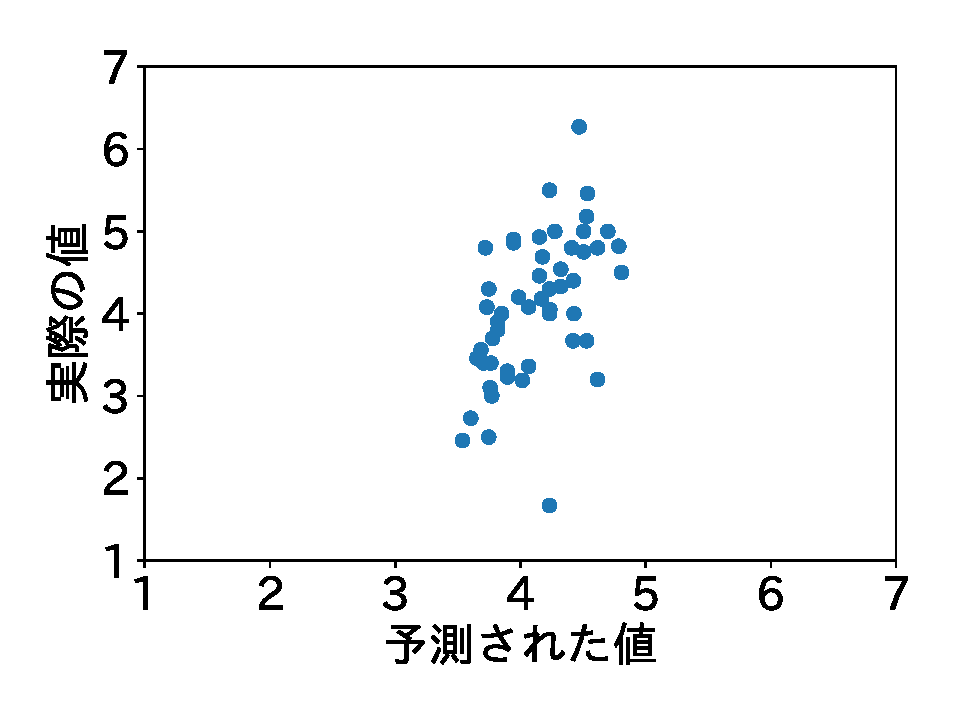
\includegraphics[width=0.4\linewidth]{fig/scatter/4.pdf}}
  \hspace{3mm}
  \subcaptionbox{声の強さ}{
  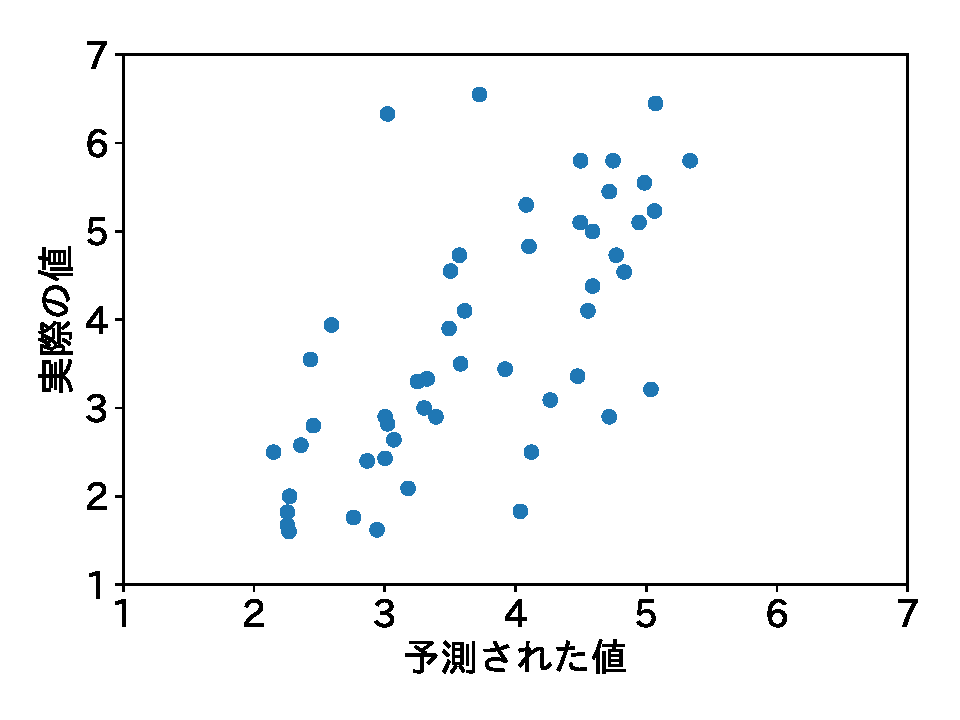
\includegraphics[width=0.4\linewidth]{fig/scatter/5.pdf}}
  \vspace{3mm}
  \subcaptionbox{声の明度}{
  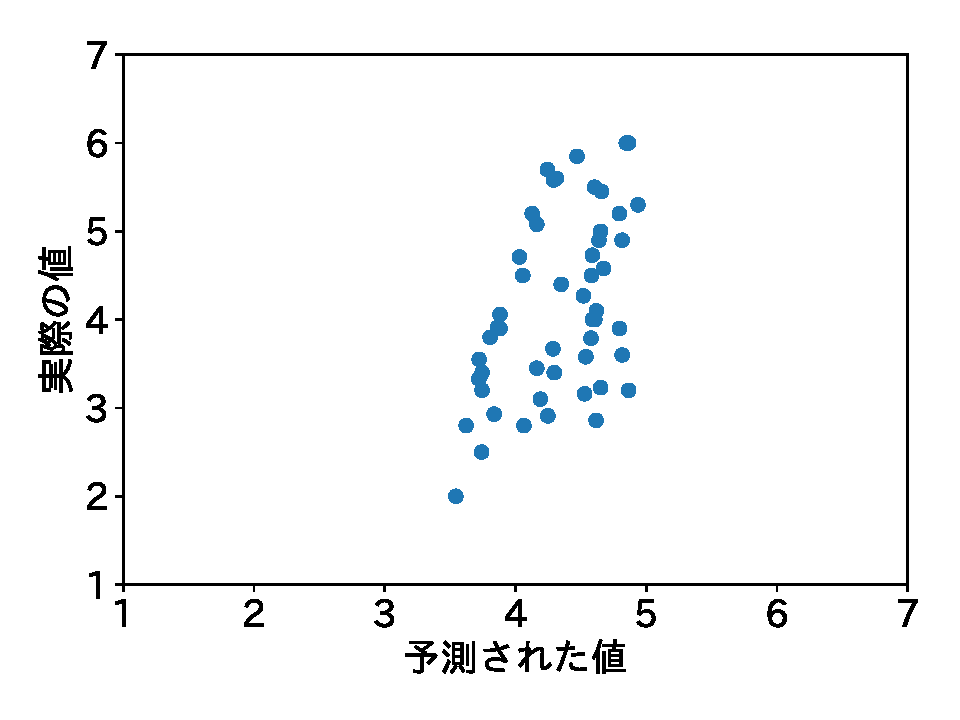
\includegraphics[width=0.4\linewidth]{fig/scatter/6.pdf}}
  \caption{実際の値と推測された値の散布図}
  \label{fig:scatters}
\end{figure}

% Local Variables:
% mode: japanese-LaTeX
% TeX-master: "root"
% End:
